\documentclass{standalone}
\usepackage{tikz}
\usetikzlibrary{patterns, positioning}


\begin{document}
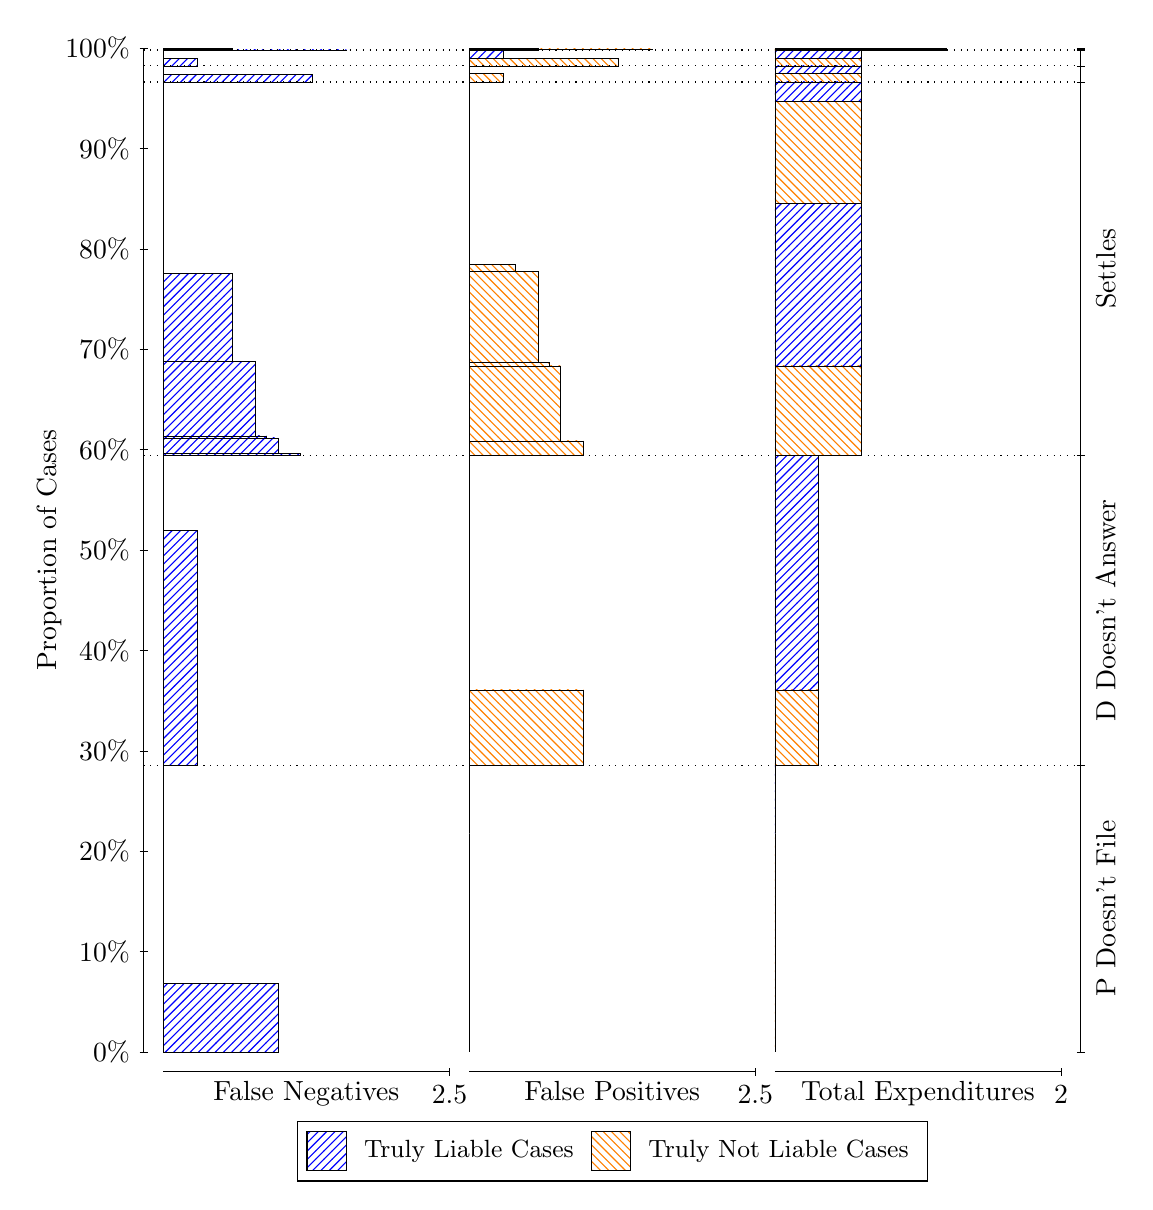
\begin{tikzpicture}
\draw[black, very thin] (1.5,1.75) -- (1.5,14.5);
\node[rotate=90, text=black, anchor=center] at (0.3, 8.125) {Proportion of Cases};
\draw[black, very thin] (1.45,1.75) -- (1.55,1.75);
\node[text=black, anchor=east] at (1.45, 1.75) {0\%};
\draw[black, very thin] (1.45,3.025) -- (1.55,3.025);
\node[text=black, anchor=east] at (1.45, 3.025) {10\%};
\draw[black, very thin] (1.45,4.3) -- (1.55,4.3);
\node[text=black, anchor=east] at (1.45, 4.3) {20\%};
\draw[black, very thin] (1.45,5.575) -- (1.55,5.575);
\node[text=black, anchor=east] at (1.45, 5.575) {30\%};
\draw[black, very thin] (1.45,6.85) -- (1.55,6.85);
\node[text=black, anchor=east] at (1.45, 6.85) {40\%};
\draw[black, very thin] (1.45,8.125) -- (1.55,8.125);
\node[text=black, anchor=east] at (1.45, 8.125) {50\%};
\draw[black, very thin] (1.45,9.4) -- (1.55,9.4);
\node[text=black, anchor=east] at (1.45, 9.4) {60\%};
\draw[black, very thin] (1.45,10.675) -- (1.55,10.675);
\node[text=black, anchor=east] at (1.45, 10.675) {70\%};
\draw[black, very thin] (1.45,11.95) -- (1.55,11.95);
\node[text=black, anchor=east] at (1.45, 11.95) {80\%};
\draw[black, very thin] (1.45,13.225) -- (1.55,13.225);
\node[text=black, anchor=east] at (1.45, 13.225) {90\%};
\draw[black, very thin] (1.45,14.5) -- (1.55,14.5);
\node[text=black, anchor=east] at (1.45, 14.5) {100\%};

\draw[black, very thin] (13.4,1.75) -- (13.4,14.5);
\draw[black, very thin] (13.35,1.75) -- (13.45,1.75);
\node[anchor=west] at (13.35, 1.75) {};
\draw[black, very thin] (13.35,5.3929) -- (13.45,5.3929);
\node[anchor=west] at (13.35, 5.3929) {};
\draw[black, very thin] (13.35,9.3272) -- (13.45,9.3272);
\node[anchor=west] at (13.35, 9.3272) {};
\draw[black, very thin] (13.35,14.069) -- (13.45,14.069);
\node[anchor=west] at (13.35, 14.069) {};
\draw[black, very thin] (13.35,14.273) -- (13.45,14.273);
\node[anchor=west] at (13.35, 14.273) {};
\draw[black, very thin] (13.35,14.47) -- (13.45,14.47);
\node[anchor=west] at (13.35, 14.47) {};
\draw[black, very thin] (13.35,14.485) -- (13.45,14.485);
\node[anchor=west] at (13.35, 14.485) {};
\draw[black, very thin] (13.35,14.5) -- (13.45,14.5);
\node[anchor=west] at (13.35, 14.5) {};

\draw[black, very thin, pattern color=blue, pattern=north east lines] (1.75,1.75) rectangle (3.2033,2.6196);
\draw[black, very thin, pattern color=orange, pattern=north west lines] (1.75,2.6196) rectangle (1.75,5.3929);
\draw[black, very thin, pattern color=blue, pattern=north east lines] (1.75,5.3929) rectangle (2.186,8.3714);
\draw[black, very thin, pattern color=orange, pattern=north west lines] (1.75,8.3714) rectangle (1.75,9.3272);
\draw[black, very thin, pattern color=blue, pattern=north east lines] (1.75,9.3272) rectangle (3.494,9.3527);
\draw[black, very thin, pattern color=blue, pattern=north east lines] (1.75,9.3527) rectangle (3.2033,9.5497);
\draw[black, very thin, pattern color=blue, pattern=north east lines] (1.75,9.5497) rectangle (3.058,9.5731);
\draw[black, very thin, pattern color=blue, pattern=north east lines] (1.75,9.5731) rectangle (2.9127,10.523);
\draw[black, very thin, pattern color=blue, pattern=north east lines] (1.75,10.523) rectangle (2.622,11.64);
\draw[black, very thin, pattern color=orange, pattern=north west lines] (1.75,11.64) rectangle (1.75,14.069);
\draw[black, very thin, pattern color=blue, pattern=north east lines] (1.75,14.069) rectangle (3.6393,14.169);
\draw[black, very thin, pattern color=orange, pattern=north west lines] (1.75,14.169) rectangle (1.75,14.273);
\draw[black, very thin, pattern color=blue, pattern=north east lines] (1.75,14.273) rectangle (2.186,14.372);
\draw[black, very thin, pattern color=orange, pattern=north west lines] (1.75,14.372) rectangle (1.75,14.47);
\draw[black, very thin, pattern color=blue, pattern=north east lines] (1.75,14.47) rectangle (4.0753,14.475);
\draw[black, very thin, pattern color=orange, pattern=north west lines] (1.75,14.475) rectangle (1.75,14.485);
\draw[black, very thin, pattern color=blue, pattern=north east lines] (1.75,14.485) rectangle (2.622,14.495);
\draw[black, very thin, pattern color=orange, pattern=north west lines] (1.75,14.495) rectangle (1.75,14.5);
\draw[black, very thin, pattern color=orange, pattern=north west lines] (5.6333,1.75) rectangle (5.6333,4.5233);
\draw[black, very thin, pattern color=blue, pattern=north east lines] (5.6333,4.5233) rectangle (5.6333,5.3929);
\draw[black, very thin, pattern color=orange, pattern=north west lines] (5.6333,5.3929) rectangle (7.0867,6.3487);
\draw[black, very thin, pattern color=blue, pattern=north east lines] (5.6333,6.3487) rectangle (5.6333,9.3272);
\draw[black, very thin, pattern color=orange, pattern=north west lines] (5.6333,9.3272) rectangle (7.0867,9.5094);
\draw[black, very thin, pattern color=orange, pattern=north west lines] (5.6333,9.5094) rectangle (6.796,10.463);
\draw[black, very thin, pattern color=orange, pattern=north west lines] (5.6333,10.463) rectangle (6.6507,10.509);
\draw[black, very thin, pattern color=orange, pattern=north west lines] (5.6333,10.509) rectangle (6.5053,11.663);
\draw[black, very thin, pattern color=orange, pattern=north west lines] (5.6333,11.663) rectangle (6.2147,11.757);
\draw[black, very thin, pattern color=blue, pattern=north east lines] (5.6333,11.757) rectangle (5.6333,14.069);
\draw[black, very thin, pattern color=orange, pattern=north west lines] (5.6333,14.069) rectangle (6.0693,14.174);
\draw[black, very thin, pattern color=blue, pattern=north east lines] (5.6333,14.174) rectangle (5.6333,14.273);
\draw[black, very thin, pattern color=orange, pattern=north west lines] (5.6333,14.273) rectangle (7.5227,14.37);
\draw[black, very thin, pattern color=blue, pattern=north east lines] (5.6333,14.37) rectangle (6.0693,14.47);
\draw[black, very thin, pattern color=orange, pattern=north west lines] (5.6333,14.47) rectangle (6.5053,14.48);
\draw[black, very thin, pattern color=blue, pattern=north east lines] (5.6333,14.48) rectangle (5.6333,14.485);
\draw[black, very thin, pattern color=orange, pattern=north west lines] (5.6333,14.485) rectangle (7.9587,14.489);
\draw[black, very thin, pattern color=blue, pattern=north east lines] (5.6333,14.489) rectangle (6.5053,14.5);
\draw[black, very thin, pattern color=orange, pattern=north west lines] (9.5167,1.75) rectangle (9.5167,4.5233);
\draw[black, very thin, pattern color=blue, pattern=north east lines] (9.5167,4.5233) rectangle (9.5167,5.3929);
\draw[black, very thin, pattern color=orange, pattern=north west lines] (9.5167,5.3929) rectangle (10.062,6.3487);
\draw[black, very thin, pattern color=blue, pattern=north east lines] (9.5167,6.3487) rectangle (10.062,9.3272);
\draw[black, very thin, pattern color=orange, pattern=north west lines] (9.5167,9.3272) rectangle (10.607,10.463);
\draw[black, very thin, pattern color=blue, pattern=north east lines] (9.5167,10.463) rectangle (10.607,12.53);
\draw[black, very thin, pattern color=orange, pattern=north west lines] (9.5167,12.53) rectangle (10.607,13.823);
\draw[black, very thin, pattern color=blue, pattern=north east lines] (9.5167,13.823) rectangle (10.607,14.069);
\draw[black, very thin, pattern color=orange, pattern=north west lines] (9.5167,14.069) rectangle (10.607,14.174);
\draw[black, very thin, pattern color=blue, pattern=north east lines] (9.5167,14.174) rectangle (10.607,14.273);
\draw[black, very thin, pattern color=orange, pattern=north west lines] (9.5167,14.273) rectangle (10.607,14.37);
\draw[black, very thin, pattern color=blue, pattern=north east lines] (9.5167,14.37) rectangle (10.607,14.47);
\draw[black, very thin, pattern color=orange, pattern=north west lines] (9.5167,14.47) rectangle (11.697,14.48);
\draw[black, very thin, pattern color=blue, pattern=north east lines] (9.5167,14.48) rectangle (11.697,14.485);
\draw[black, very thin, pattern color=orange, pattern=north west lines] (9.5167,14.485) rectangle (11.697,14.489);
\draw[black, very thin, pattern color=blue, pattern=north east lines] (9.5167,14.489) rectangle (11.697,14.5);
\draw[black, dotted] (1.5,5.3929) -- (13.4,5.3929);
\draw[black, dotted] (1.5,9.3272) -- (13.4,9.3272);
\draw[black, dotted] (1.5,14.069) -- (13.4,14.069);
\draw[black, dotted] (1.5,14.273) -- (13.4,14.273);
\draw[black, dotted] (1.5,14.47) -- (13.4,14.47);
\draw[black, dotted] (1.5,14.485) -- (13.4,14.485);
\draw[black, very thin] (1.75,1.5) -- (5.3833,1.5);
\node[text=black, anchor=north] at (3.5667, 1.5) {False Negatives};
\draw[black, very thin] (5.3833,1.45) -- (5.3833,1.55);
\node[text=black, anchor=north] at (5.3833, 1.45) {2.5};

\draw[black, very thin] (5.6333,1.5) -- (9.2667,1.5);
\node[text=black, anchor=north] at (7.45, 1.5) {False Positives};
\draw[black, very thin] (9.2667,1.45) -- (9.2667,1.55);
\node[text=black, anchor=north] at (9.2667, 1.45) {2.5};

\draw[black, very thin] (9.5167,1.5) -- (13.15,1.5);
\node[text=black, anchor=north] at (11.333, 1.5) {Total Expenditures};
\draw[black, very thin] (13.15,1.45) -- (13.15,1.55);
\node[text=black, anchor=north] at (13.15, 1.45) {2};

\node[text=black, centered, rotate=90] at (13.72, 3.5714) {P Doesn't File};
\node[text=black, centered, rotate=90] at (13.72, 7.36) {D Doesn't Answer};
\node[text=black, centered, rotate=90] at (13.72, 11.698) {Settles};





\draw (7.449999999999999,1.5) node[draw=none] (baseCoordinate) {};
\begin{scope}[align=center]
        \matrix[scale=0.5, draw=black, below=0.5cm of baseCoordinate, nodes={draw}, column sep=0.1cm]{
            \node[rectangle, draw, minimum width=0.5cm, minimum height=0.5cm, pattern color=blue, pattern=north east lines] {}; &
            \node[draw=none, font=\small, text=black] (B) {Truly Liable Cases}; &
            \node[rectangle, draw, minimum width=0.5cm, minimum height=0.5cm, pattern color=orange, pattern=north west lines] {}; &
            \node[draw=none, font=\small, text=black] (B) {Truly Not Liable Cases}; \\
            };
\end{scope}

\end{tikzpicture}
\end{document}